\documentclass{beamer}

%%%%%%%%%%%%%%%%%%%%%%%%%%%%%%%%%%%%%%%%%%%%%%%%%%%%%%%%%%%%%%%%
%%%                  Themes and such                         %%%
%%%%%%%%%%%%%%%%%%%%%%%%%%%%%%%%%%%%%%%%%%%%%%%%%%%%%%%%%%%%%%%%
\mode<presentation>
{
  %\usetheme{Copenhagen}  
  %\usetheme{Warsaw}  
  \usetheme{Malmoe}  
  %  \setbeamertemplate{headline}{}
  %make my huge toc fit on one slide (and not look horrible)
  %\setbeamerfont{subsection in toc}{series=\bfseries}
  %\setbeamerfont{subsection in toc}{size=\tiny,series=\bfseries}
}

%%%%%%%%%%%%%%%%%%%%%%%%%%%%%%%%%%%%%%%%%%%%%%%%%%%%%%%%%%%%%%%%
%%%                       Packages                           %%%
%%%%%%%%%%%%%%%%%%%%%%%%%%%%%%%%%%%%%%%%%%%%%%%%%%%%%%%%%%%%%%%%
\usepackage{multimedia}
\usepackage{multirow}
\usepackage{subfigure}
\usepackage{amsmath}
\usepackage{parskip}
\setlength{\parskip}{\smallskipamount} 
\usepackage{color}
\usepackage{tikz}
%\usepackage{tcolorbox}

% Define commands
 \newcommand{\half}{\ensuremath{\frac{1}{2}}}

 \newcommand{\bea}{\begin{eqnarray}}
 \newcommand{\eea}{\end{eqnarray}}
 \newcommand{\beq}{\begin{equation}}
 \newcommand{\eeq}{\end{equation}}
 \newcommand{\bed}{\begin{displaymath}}
 \newcommand{\eed}{\end{displaymath}}

 \newcommand{\pd}[2]{\dfrac{\partial #1}{\partial #2}}
 \newcommand{\pf}[2]{\dfrac{d #1}{d #2}}
 \newcommand{\pdt}[2]{\dfrac{\partial^2 #1}{\partial #2^2}}
 \newcommand{\pft}[2]{\dfrac{d^2 #1}{d #2^2}}
 \newcommand{\pdtno}[2]{\dfrac{\partial^2 #1}{\partial #2}}
 \newcommand{\pdd}[3]{\dfrac{\partial^2 #1}{\partial #2 \partial #3}}
 \newcommand{\pff}[3]{\dfrac{d^2 #1}{d #2 d #3}}

 \graphicspath{{../figures/}}

\makeatletter
\newenvironment{noheadline}{
    \setbeamertemplate{headline}{}
    \addtobeamertemplate{frametitle}{\vspace*{-1.5\baselineskip}}{}
}{}
\makeatother

%%%%%%%%%%%%%%%%%%%%%%%%%%%%%%%%%%%%%%%%%%%%%%%%%%%%%%%%%%%%%%%%
%%%                     Title Info                           %%%
%%%%%%%%%%%%%%%%%%%%%%%%%%%%%%%%%%%%%%%%%%%%%%%%%%%%%%%%%%%%%%%%

\title[\hspace{-0.2cm} Time Dependent Discrete Adjoint]
{
Time Dependent Discrete Adjoint Formulations for Structural Dynamics
}

\author[Komahan Boopathy]
{
  \Large {Komahan Boopathy}\\
}

\institute
{
  \large Structures and Multidisciplinary Optimization Laboratory \\
  ~\\
   Georgia Institute of Technology\\
 School of Aerospace Engineering\\
 Atlanta, GA
}

\date
{
\small \today
}

\begin{document}
\setbeamertemplate{background}{
  \begin{tikzpicture}
    \node[opacity=.1,inner sep=0pt]{
     
\includegraphics [height=\paperheight]{gt.png}};
  \end{tikzpicture}
}
% Now we install the new template for the following frames:
%\usebackgroundtemplate{%
%  \includegraphics[width=\paperwidth,height=\paperheight]{}}

\begin{frame}
  \titlepage
\end{frame}

\setbeamertemplate{background}{
  \begin{tikzpicture}
    \node[opacity=.03,inner sep=0pt]{
     
\includegraphics [height=\paperheight]{gt.png}};
  \end{tikzpicture}
}
%\begin{frame}
%  \frametitle{Outline}
%  \tableofcontents
%\end{frame}
\begin{noheadline}
\begin{frame}[allowframebreaks] \frametitle{Newmark--Beta--Gamma Method Adjoint}
  \tiny{

\begin{minipage}{1.0\linewidth}
\begin{block}{101. Notation:}
    \begin{tabbing}
      XXXXXX \= xxxx\kill
      $t$     \> time \\
      $k$     \> time index \\
      $x$     \> design variables \\
      $m$     \> number of design variables \\
      $u,v,w$ \> state variables \\
      $n$  \> number of state variables \\
      $R, S, T$ \> constraint governing equations  \\
      $\rho ,~ \sigma ,~\tau$ \> adjoint variables  \\
      $F$     \> objective function \\
      $\cal{L}$ \> Lagrangian \\
    \end{tabbing}
\end{block}
\end{minipage}
\begin{minipage}{1.0\linewidth}
\begin{block}{1. Objective Function:}
    A time-averaged objective function is considered (e.g. mean lift,
    mean potential energy, mean thermal-stress). We can approximate
    the integral as a discrete sum:
    \begin{equation}\label{eqn:time-averaged-function}
      F = \frac{1}{T}\int_{0}^T f_k(u,v,w,x,t)~dt=\sum_{k=0}^N h f_k(u_k,v_k,w_k,x)
    \end{equation}
    Other possibilities for the choice of objective function exist
    too.
\end{block}
\end{minipage}
\framebreak

\begin{block}{2. Optimization Problem:}
  We would like to minimize the time-dependent objective function,
  $F$, such that the governing constraint equations $(R, S, T)$ are
  satisfied at all time steps.  Mathematically, a \underline{general}
  optimization problem can be posed as follows:
  \begin{equation}
    \begin{aligned}
      & \underset{x}{\text{minimize}}
      & & F = F(u, v, w, x,t) \\
      & \text{subject to} & &  R(u, x_r, t), S(v, x_s, t), T(w, x_t, t) = 0.\\
      %        & & &  S(v) = 0,\\
      %        & &  & T(w) = 0.\\
      %& \text{bounds}
      %& & \d^\text{L} \le \d \le \d^\text{U}.
    \end{aligned}
  \end{equation}
  where $x = [x_r, x_s, x_t]$ is a vector of design variables.
\end{block}

\begin{block}{3. Lagrangian:}
  It would be nice and handy to pack all separate equations (objects)
  into one equation (object) to operate with. We introduce
  \textcolor{red}{$\rho_k$}, \textcolor{orange}{$\sigma_k$} and
  \textcolor{blue}{$\tau_k$} as the adjoint variables associated with
  each of these function objects at the each time step and the
  Lagrangian function is written as:
  \begin{equation}\label{eqn:nbg-lagrangian}
    {\cal{L}} = \textcolor{brown}{\sum_{k=0}^N h f_k} + \textcolor{red}{ \sum_{k=0}^N h \rho_k^T R_k} 
    +  \textcolor{orange}{ \sum_{k=0}^N\sigma_k^T S_k} +  \textcolor{blue}{ \sum_{k=0}^N\tau_k^T T_k}.
  \end{equation}
  The Lagrangian is nothing but a linear ``\texttt{\underline{F}AXPY}'' 
  operator  (why not!) operating on vector objects -- just like \texttt{\underline{S}AXPY}, 
  \texttt{\underline{D}AXPY}, \texttt{\underline{Z}AXPY} (being Fortranic).
  Here $\rho,~\tau,~\sigma$ adjoint variables: they
  manifest themselves as simple-scaling-scalars in linear-algebra and
  as Lagrange multipliers in the context of optimization.
\end{block}


\framebreak

\begin{block}{4. Adjoint Variables:}
  This involves two main steps:
  \begin{enumerate}
  \item Forward mode for finding the state variables involving non-linear solves (2/3 of the
    computational time)
  \item Reverse mode for finding the adjoint variables involving
    linear-solves (1/3 of the computational time). The
    conditions $$\textcolor{red}{\pd{\cal{L}}{u_k}},
    \textcolor{orange}{\pd{\cal{L}}{v_k}},
    \textcolor{blue}{\pd{\cal{L}}{w_k}} = 0$$ can be used to generate
    a typically coupled system of equations to solve for the adjoint
    variables, $\textcolor{red}{\rho}$, $\textcolor{orange}{\sigma}$
    and $\textcolor{blue}{\tau}$. We will get three vectors of
    equations for the three vectors of adjoint variable
    unknowns. Possibilities for decoupling the system exist -- case by
    case basis. When decoupling is possible one or more of the
    constraint equations fold into other equations and therefore the
    corresponging adjoint variable need not be included in the
    formulation of the Lagrangian, but is typically done for the sake
    of generality.
  \end{enumerate}
\end{block}

  \begin{block}{5. Total Derivative:}
    The total derivative can be
    written as a \underline{linear combination} of contributions from the function
    of interest and the constraints:
    \begin{equation}\label{eqn:nbg-total-derivative}
      \pd{\cal{L}}{x} = \pd{F}{x} = 
      \textcolor{brown}{\sum_{k=0}^N h \pd{f_k}{x}^T} + 
      \textcolor{red}{\sum_{k=0}^N h \pd{R_k}{x}^T \rho_k} + 
      \textcolor{orange}{\sum_{k=0}^N \pd{S_k}{x}^T \sigma_k} + 
      \textcolor{blue}{\sum_{k=0}^N \pd{T_k}{x}^T \tau_k}.
    \end{equation}
  \end{block}
  %The projections of every other vector is used to 
  The objective function value $F$ and the gradient $\pd{F}{x}$ goes
  to the optimization code.

  \framebreak

  \begin{block}{Context of Structural Dynamics and Time Marching}
    \begin{minipage}{0.45\linewidth}
      \begin{tabbing}
        XXXXXX \= xxxx\kill
        $t$     \> time \\
        $k$     \> time index \\
        $x$     \> design variables \\
        $m$     \> number of design variables \\
        \colorbox{blue!20}{$u,v,w$} \> \colorbox{blue!20}{state variables} \\
        $n$  \> number of state variables \\
         \colorbox{green!20}{$R, S, T$} \> constraint governing equations  \\
        $\rho ,~ \sigma ,~\tau$ \> adjoint variables  \\
        $F$     \> objective function \\
        $\cal{L}$ \> Lagrangian \\
      \end{tabbing}
    \end{minipage}\hfill
    \begin{minipage}{0.45\linewidth}
      \begin{tabbing}
        XXXXXX \= xxxx\kill
        $t$     \> time \\
        $k$     \> time index \\
        $x$     \> design variables \\
        $m$     \> number of design variables \\
        \colorbox{blue!20}{$q,\dot{q},\ddot{q}$} \> \colorbox{blue!20}{position, velocity and acceleration states} \\
        $n$  \> number of state variables \\
        \colorbox{green!20}{$R, S, T$} \> constraint governing equations  \\
        $\rho ,~ \sigma ,~\tau$ \> adjoint variables  \\
        $F$     \> objective function \\
        $\cal{L}$ \> Lagrangian \\
      \end{tabbing}
    \end{minipage}
  \end{block}

    The residual of the governing equations from structural dynamics
    can be posed as: 
    \begin{equation}\label{eqn:nbg-residual}
      \textcolor{red}{R_k = R_k(\underline{\ddot{q}_k}, \dot{q}_k, q_k, x) = 0}.
    \end{equation}
    \textbf{Example:} $R = m\ddot{q} + c\dot{q} + k{q} = 0$, x = $[m,
      c, k]$ can be the design variables of choice, the objective be
    minimizing the time-averaged potential energy $F = \frac{1}{T}
    \int_{0}^T f_k~dt$, where $f_k = \frac{1}{2} kq^2$ is the
    instantaneous PE.

    \begin{minipage}{0.6\linewidth}
      We use \textbf{Newmark--Beta--Gamma (NBG)} time-marching method to
      integrate and solve for the states over time.  The states
      approximation equations are:
      \begin{equation}\label{eqn:nbg-approx-qdot}
        \textcolor{orange}{S_k =  \dot{q}_{k-1}  + (1-\gamma) h \ddot{q}_{k-1} +  \gamma h \ddot{q}_{k}- \dot{q}_k=0, }
      \end{equation}
      \begin{equation}\label{eqn:nbg-approx-q}
        \textcolor{blue}{T_k = {q}_{k-1} + h \dot{q}_{k-1} +\frac{1-2\beta}{2}
          h^2\ddot{q}_{k-1} + \beta h^2 \ddot{q}_k-{q}_k=0}. 
      \end{equation}
      The underlined varibles are the primary variables in each equation.
    \end{minipage}
    \begin{minipage}{0.39\linewidth}
      \begin{figure}
        \centering
        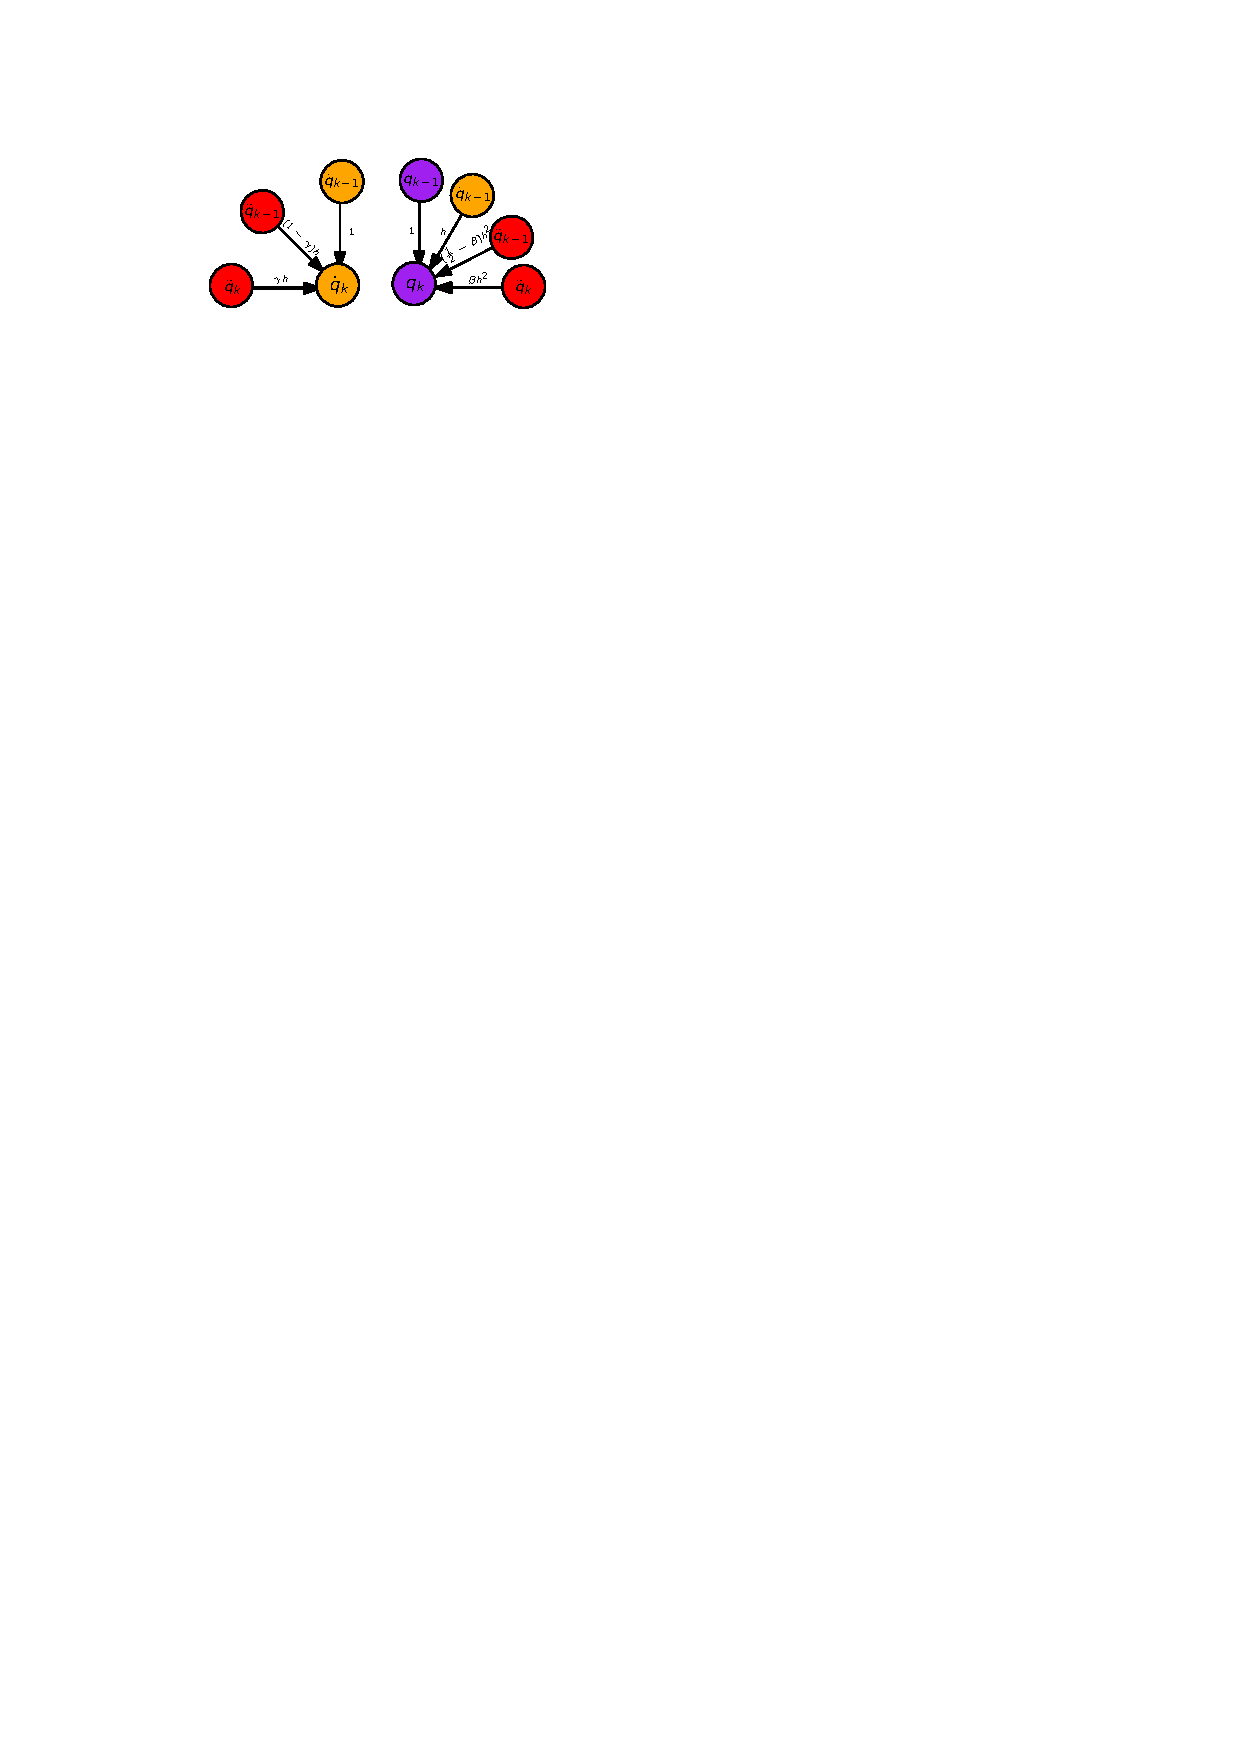
\includegraphics[width=\textwidth]{nbg-node.pdf}
        %\caption{Illustrations showing the working of NBG method.}
        \label{fig:nbg-illustration}
      \end{figure}
    \end{minipage}
    
    Eq~\eqref{eqn:nbg-residual} comes from the governing physics of
    the system. Eqs.~\eqref{eqn:nbg-approx-qdot} and
    ~\eqref{eqn:nbg-approx-q} come from the time-marching
    scheme. Therefore, the equations $S_k$ and $T_k$ are independent
    of the design variables $x$ -- they do not contribute to the total
    derivative:
    \begin{equation}\label{eqn:nbg-total-derivative}
      \pd{\cal{L}}{x} = \pd{F}{x} = \textcolor{brown}{\sum_{k=0}^N h \pd{f_k}{x}^T} +\textcolor{red}{ \sum_{k=0}^N h
    \pd{R_k}{x}^T \rho_k}.
    \end{equation}

    The conditions $$\textcolor{red}{\pd{\cal{L}}{{q}_k}},
    \textcolor{orange}{\pd{\cal{L}}{\dot{q}_k}},
    \textcolor{blue}{\pd{\cal{L}}{\ddot{q}_k}} = 0$$ can be used to
    generate a coupled system of equations to solve
    \underline{simultaneously} for the adjoint variables at each time
    step. Since the equations $S_k$ and $T_k$ are explicit, it becomes
    possible to solve \underline{sequentially} for the adjoint
    variables at each step. This property is beneficial in terms of
    reducing the size of the linear system.

    \begin{block}{Matrix Structures}

      \begin{minipage}{0.49\linewidth}
        \begin{figure}
          \centering
          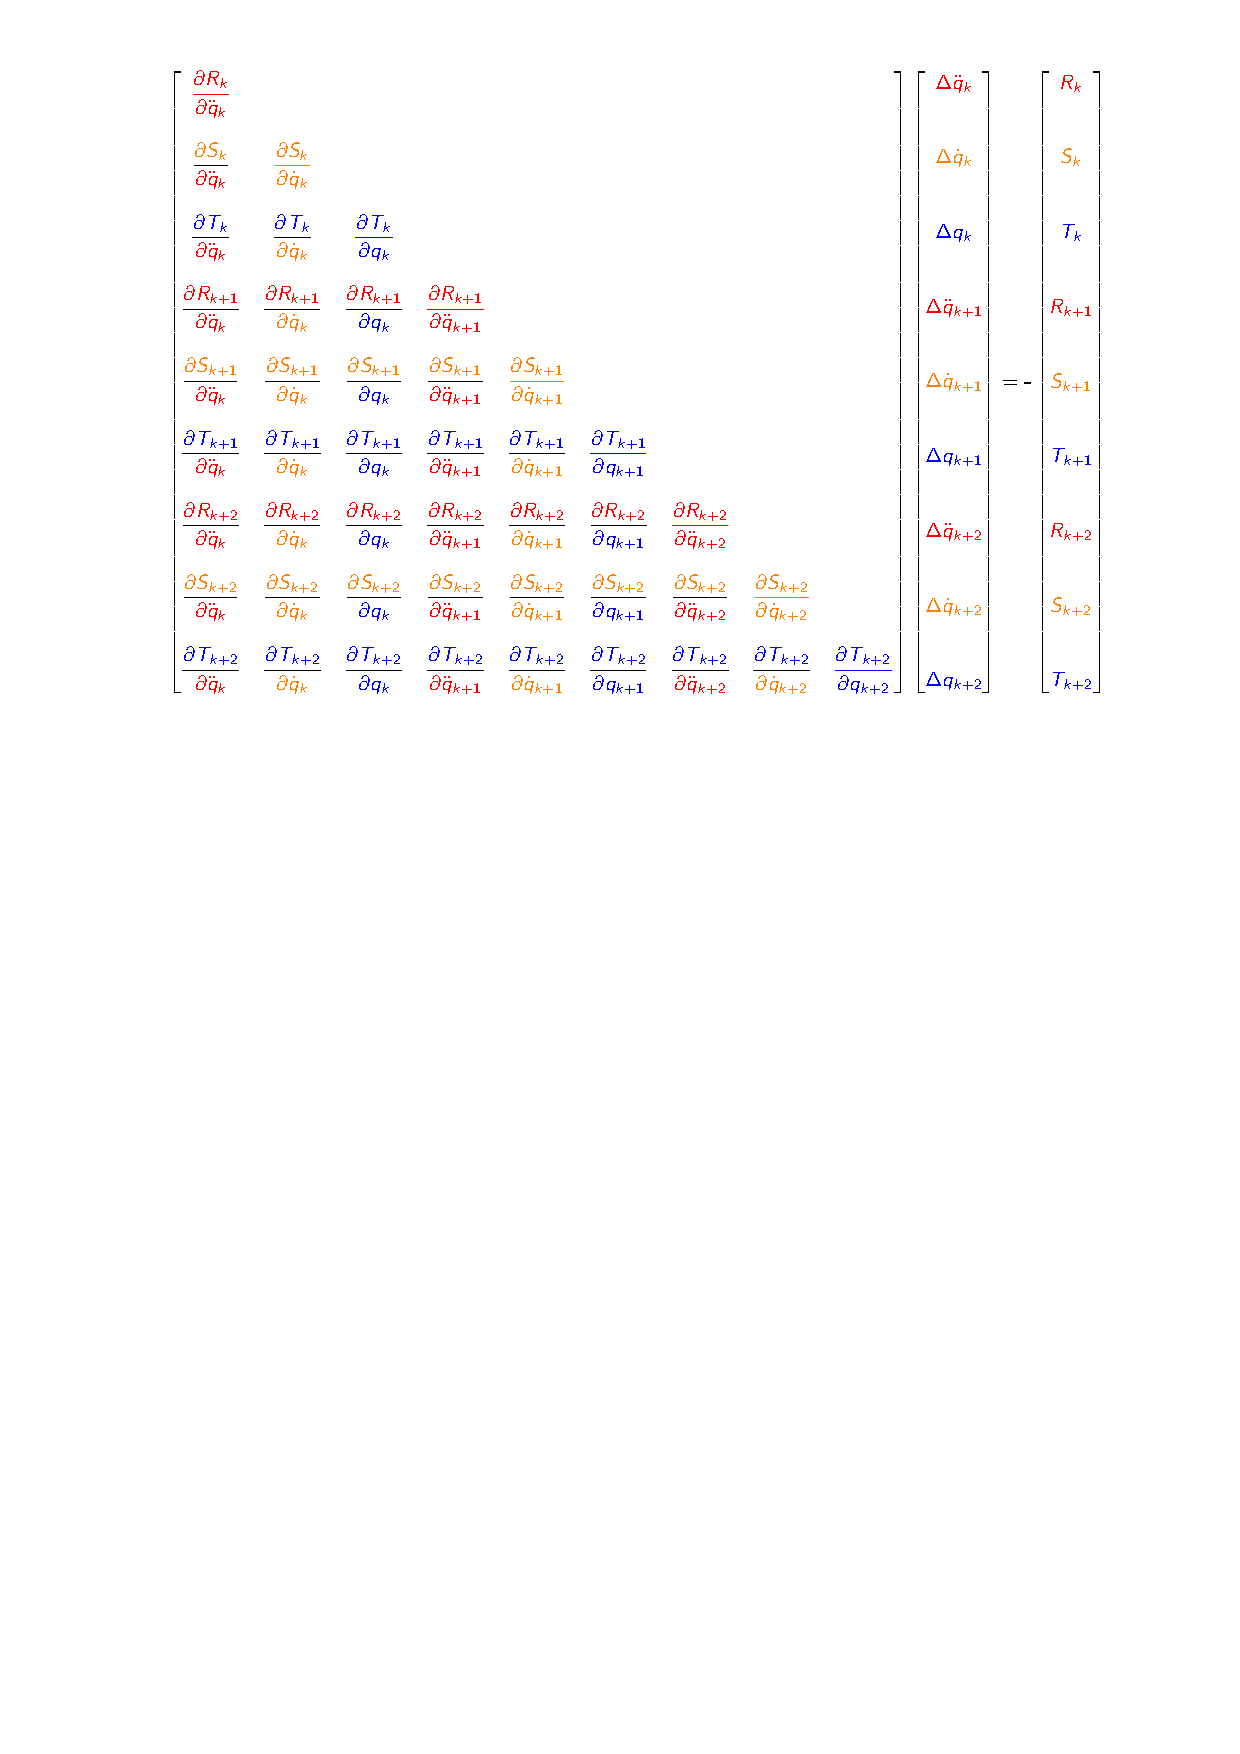
\includegraphics[width=\textwidth]{general-forward-matrix.pdf}
          \label{Forward Mode}
        \end{figure}
      \end{minipage}
      \begin{minipage}{0.49\linewidth}
        \begin{figure}
          \centering
          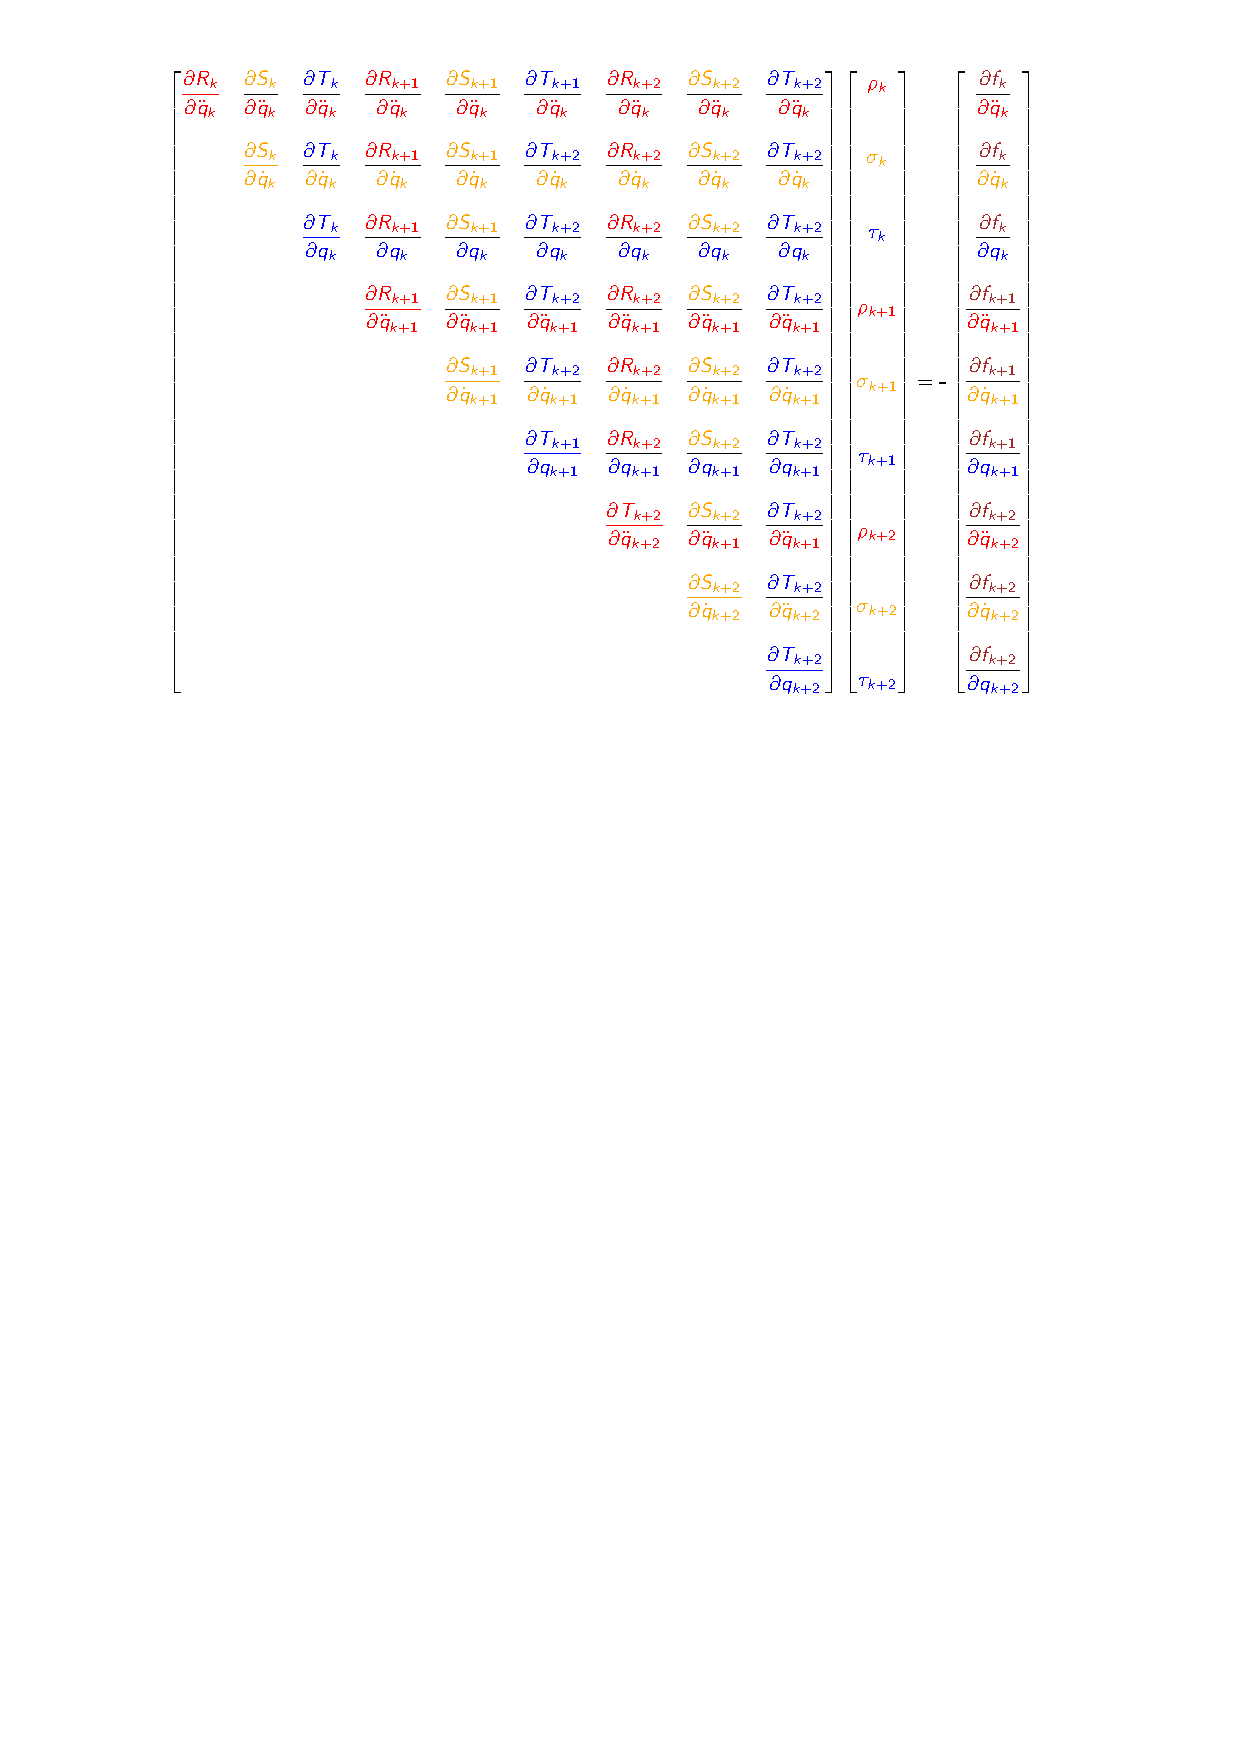
\includegraphics[width=0.925\textwidth]{general-reverse-matrix.pdf}
          \label{Reverse Mode}
        \end{figure}
      \end{minipage}

      \begin{minipage}{0.49\linewidth}
        \begin{figure}
          \centering
          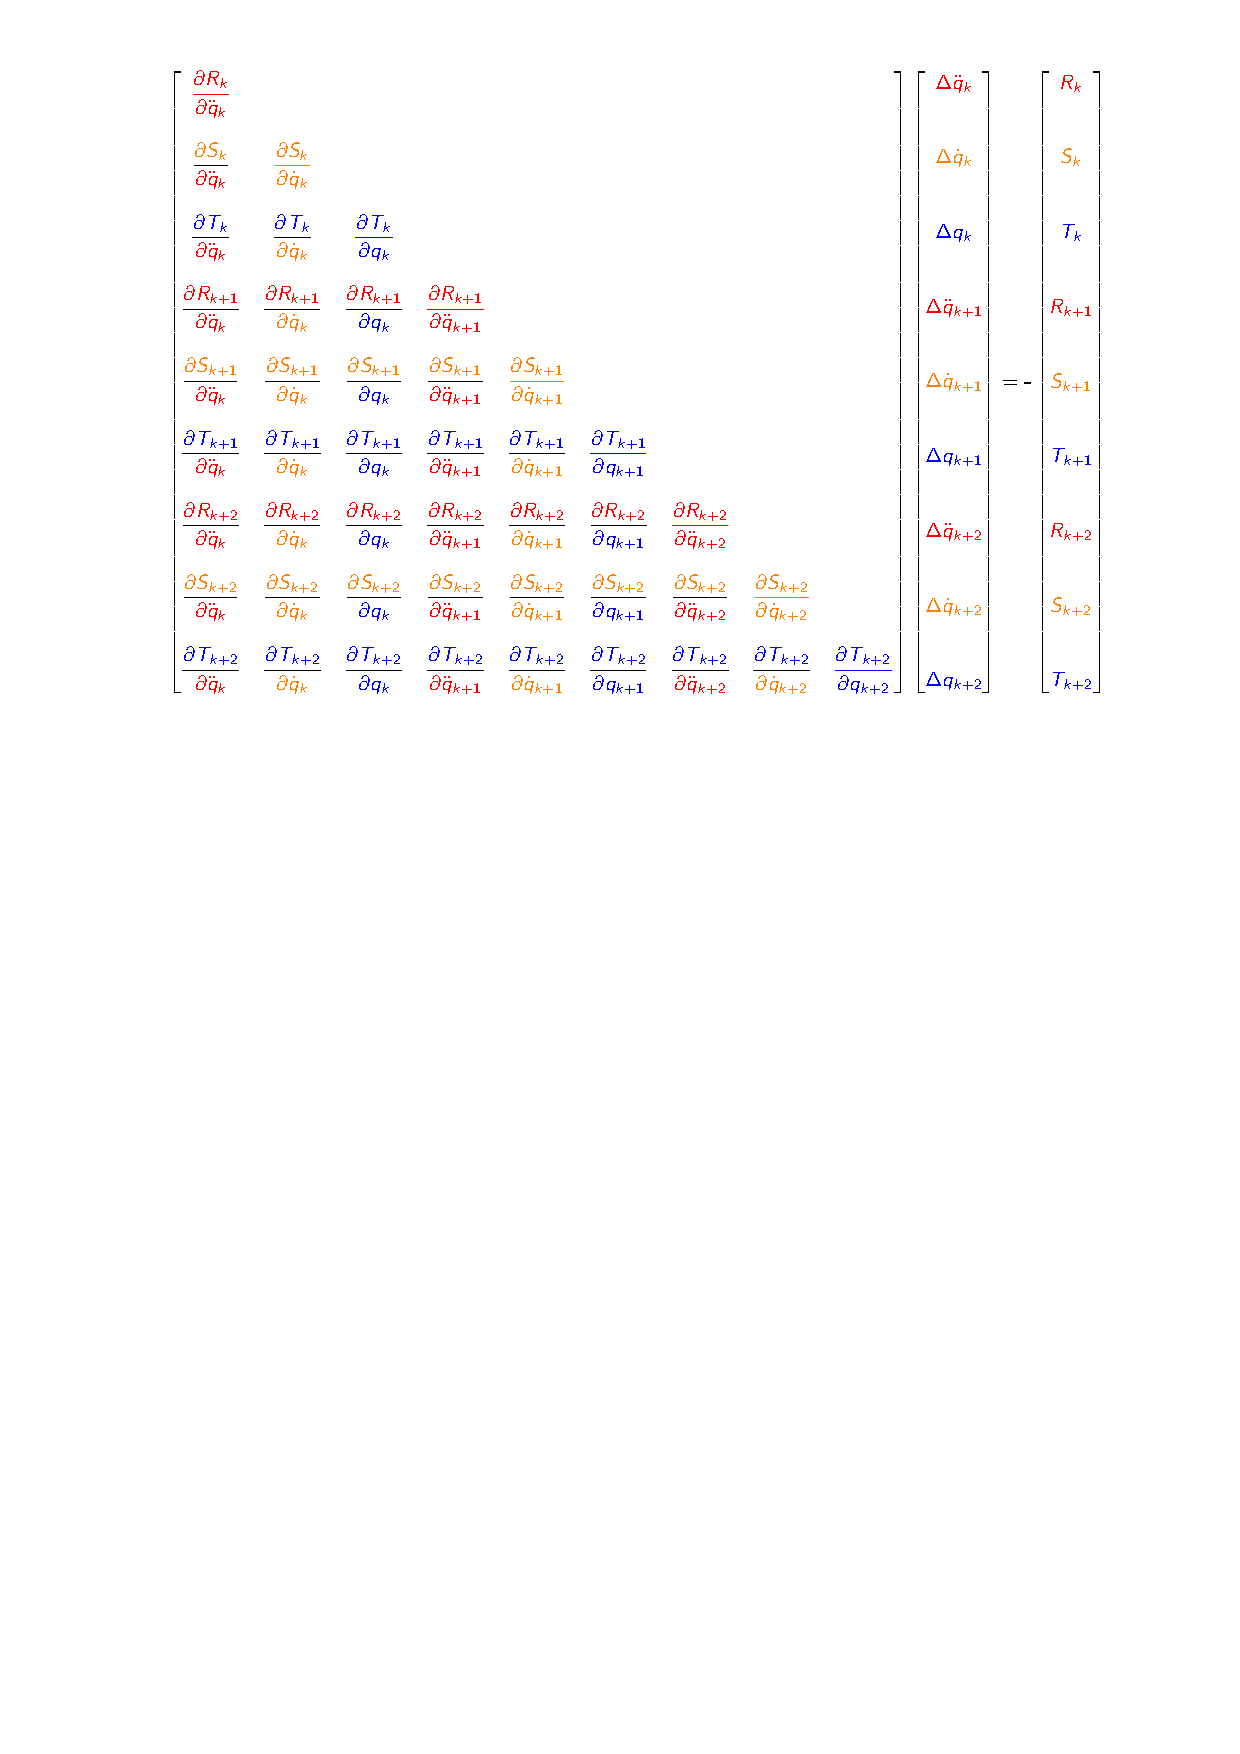
\includegraphics[width=\textwidth]{nbg-forward-matrix.pdf}
          \label{Forward Mode}
        \end{figure}
      \end{minipage}
      \begin{minipage}{0.49\linewidth}
        \begin{figure}
          \centering
          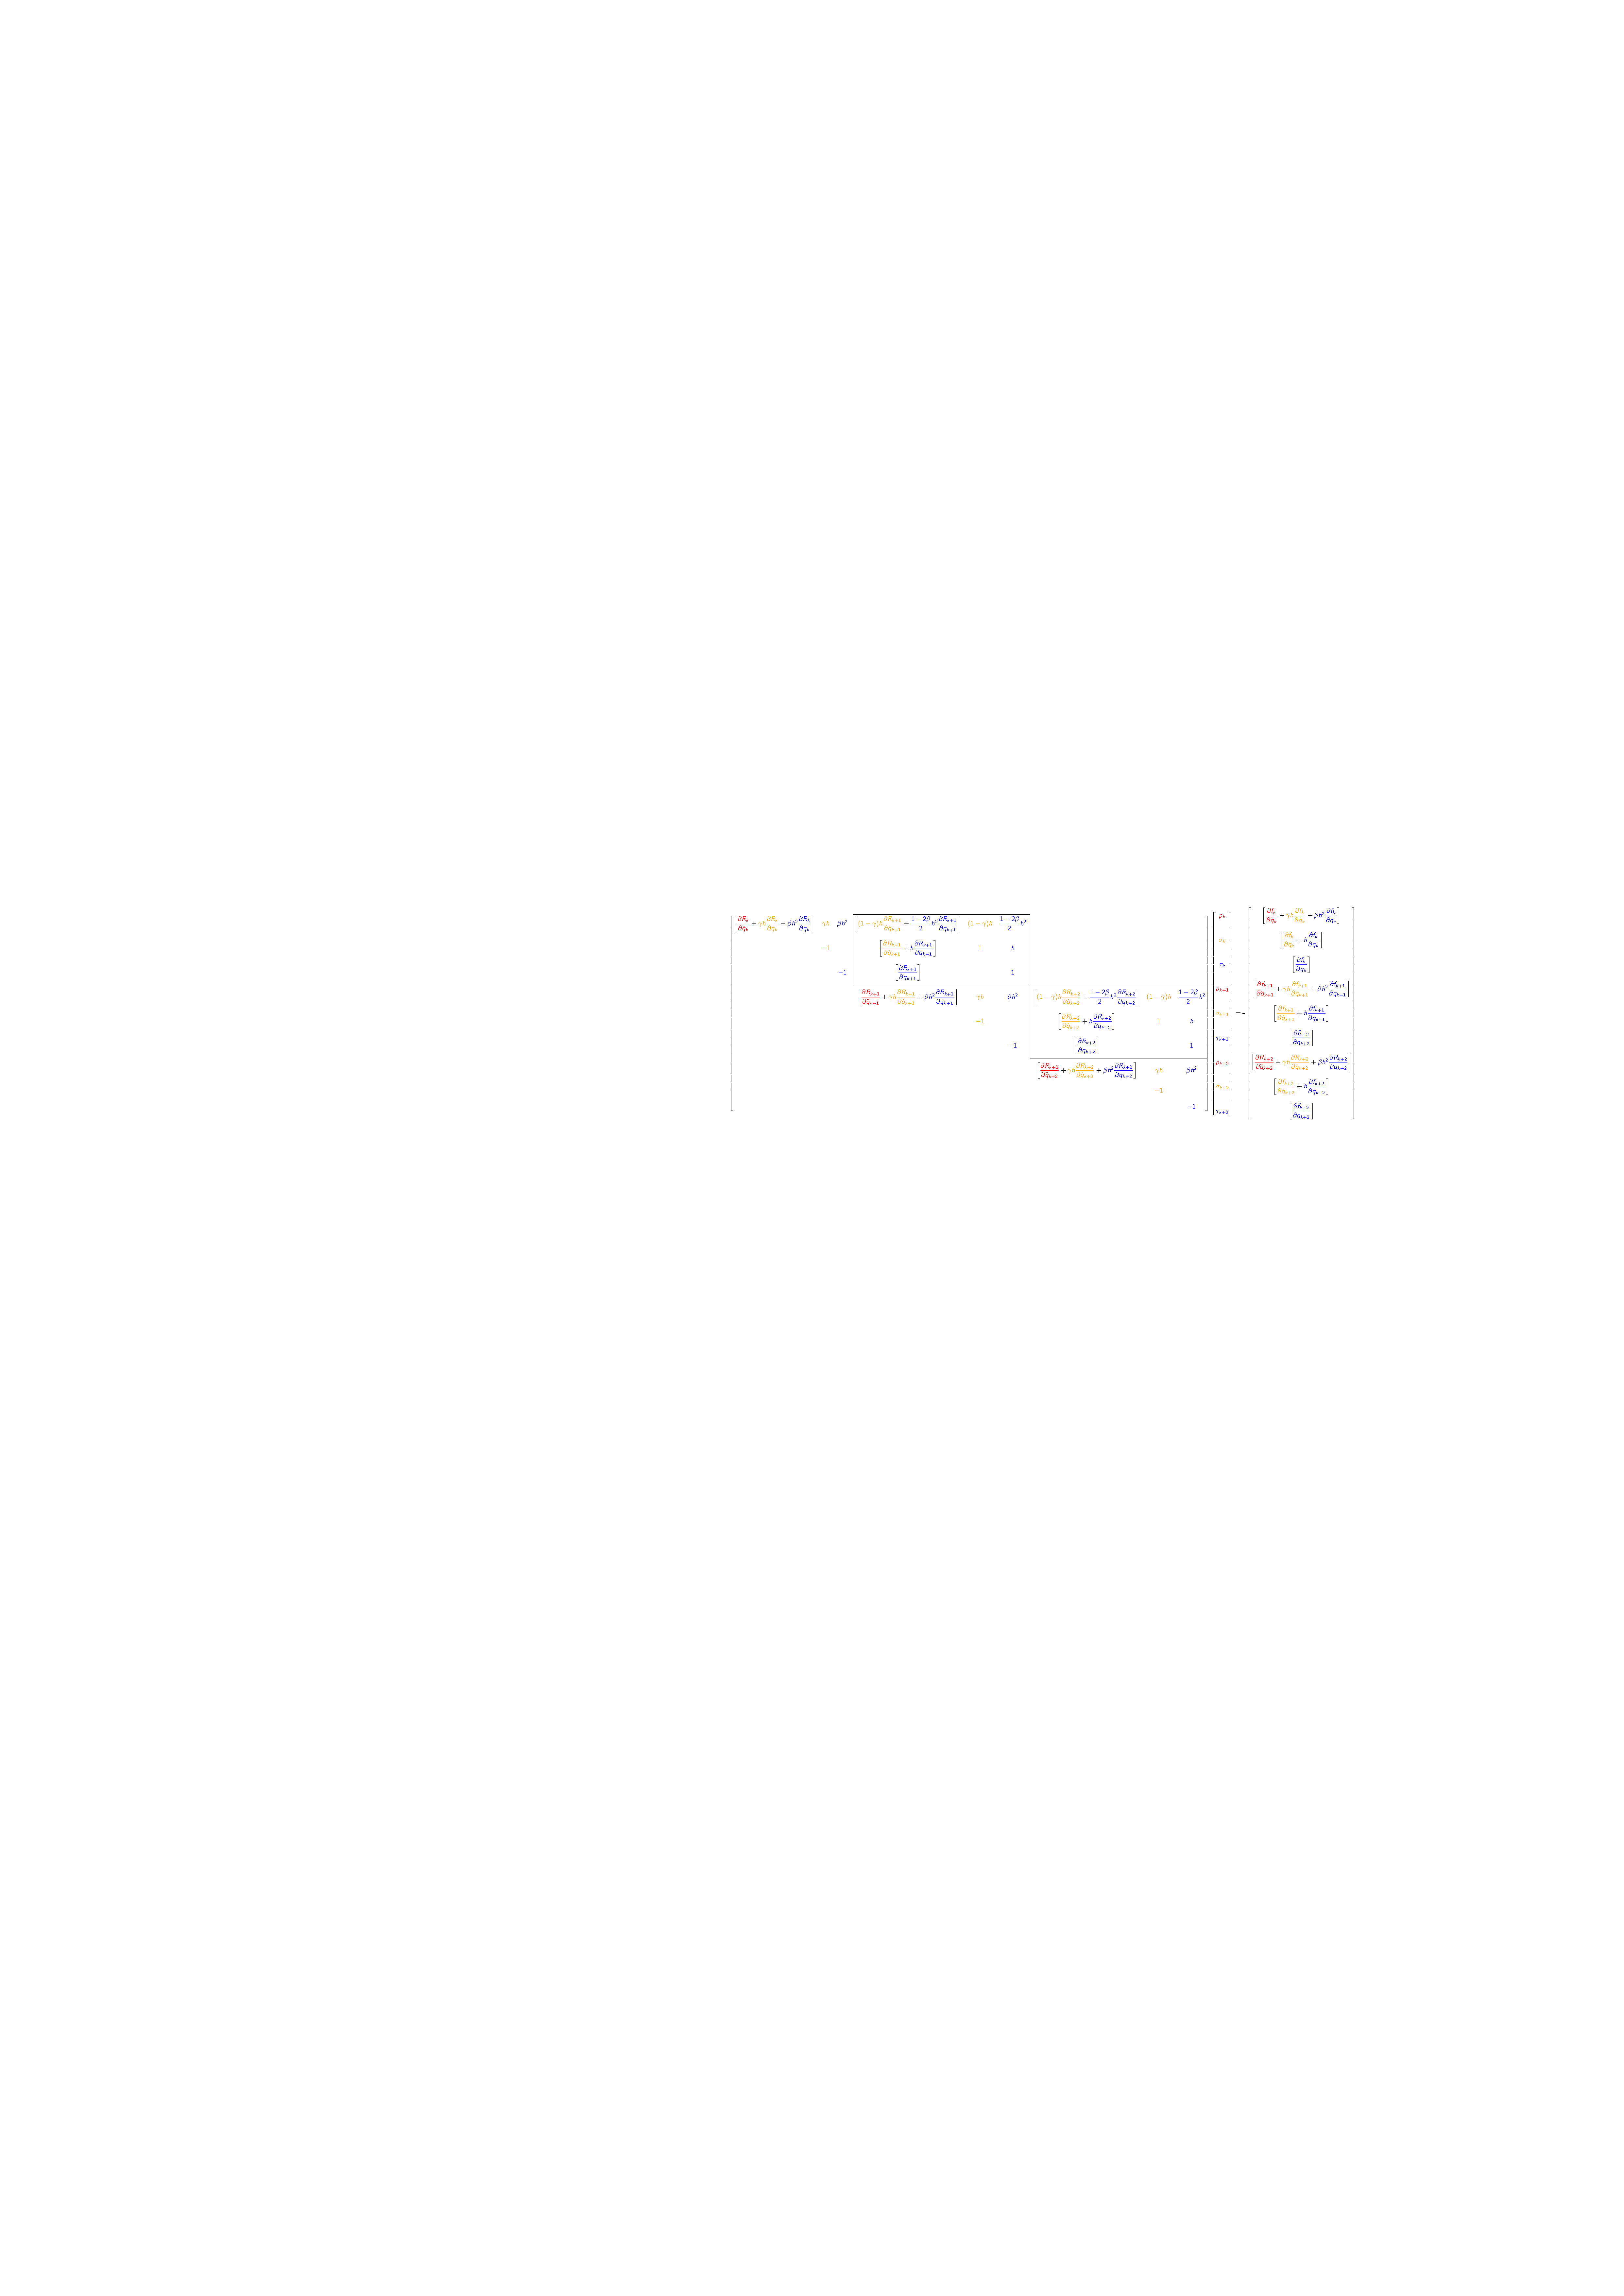
\includegraphics[width=0.925\textwidth]{nbg-reverse-matrix.pdf}
          \label{Reverse Mode}
        \end{figure}
      \end{minipage}
    \end{block}

    The steps involved are detailed as follows.  Setting
    $\pd{\cal{L}}{{q}_k} = 0$ yields:
    \begin{equation}
      \begin{split}
        \tau_k = \tau_{k+1} + \left\{h \pd{f_{k+1}}{{q}_{k+1}} \right\}^T + \left[ h \pd{R_{k+1}}{{q}_{k+1}} \right]^T \rho_{k+1}  
      \end{split}
    \end{equation}

    Setting $\pd{\cal{L}}{\dot{q}_k} = 0$ yields:
    \begin{equation}
      \begin{split}
        \sigma_k = \sigma_{k+1} + h \tau_{k+1}  + \left\{ h \pd{f_{k+1}}{\dot{q}_{k+1}} +  h^2 \pd{f_{k+1}}{{q}_{k+1}} \right\}^T + \left[ h \pd{R_{k+1}}{\dot{q}_{k+1}} +  h^2 \pd{R_{k+1}}{{q}_{k+1}} \right]^T \rho_{k+1} 
      \end{split}
    \end{equation}
    
    Figure~\ref{fig:nbg-illustration} shows the flow of information across
    states.
    \begin{figure}
      \centering
      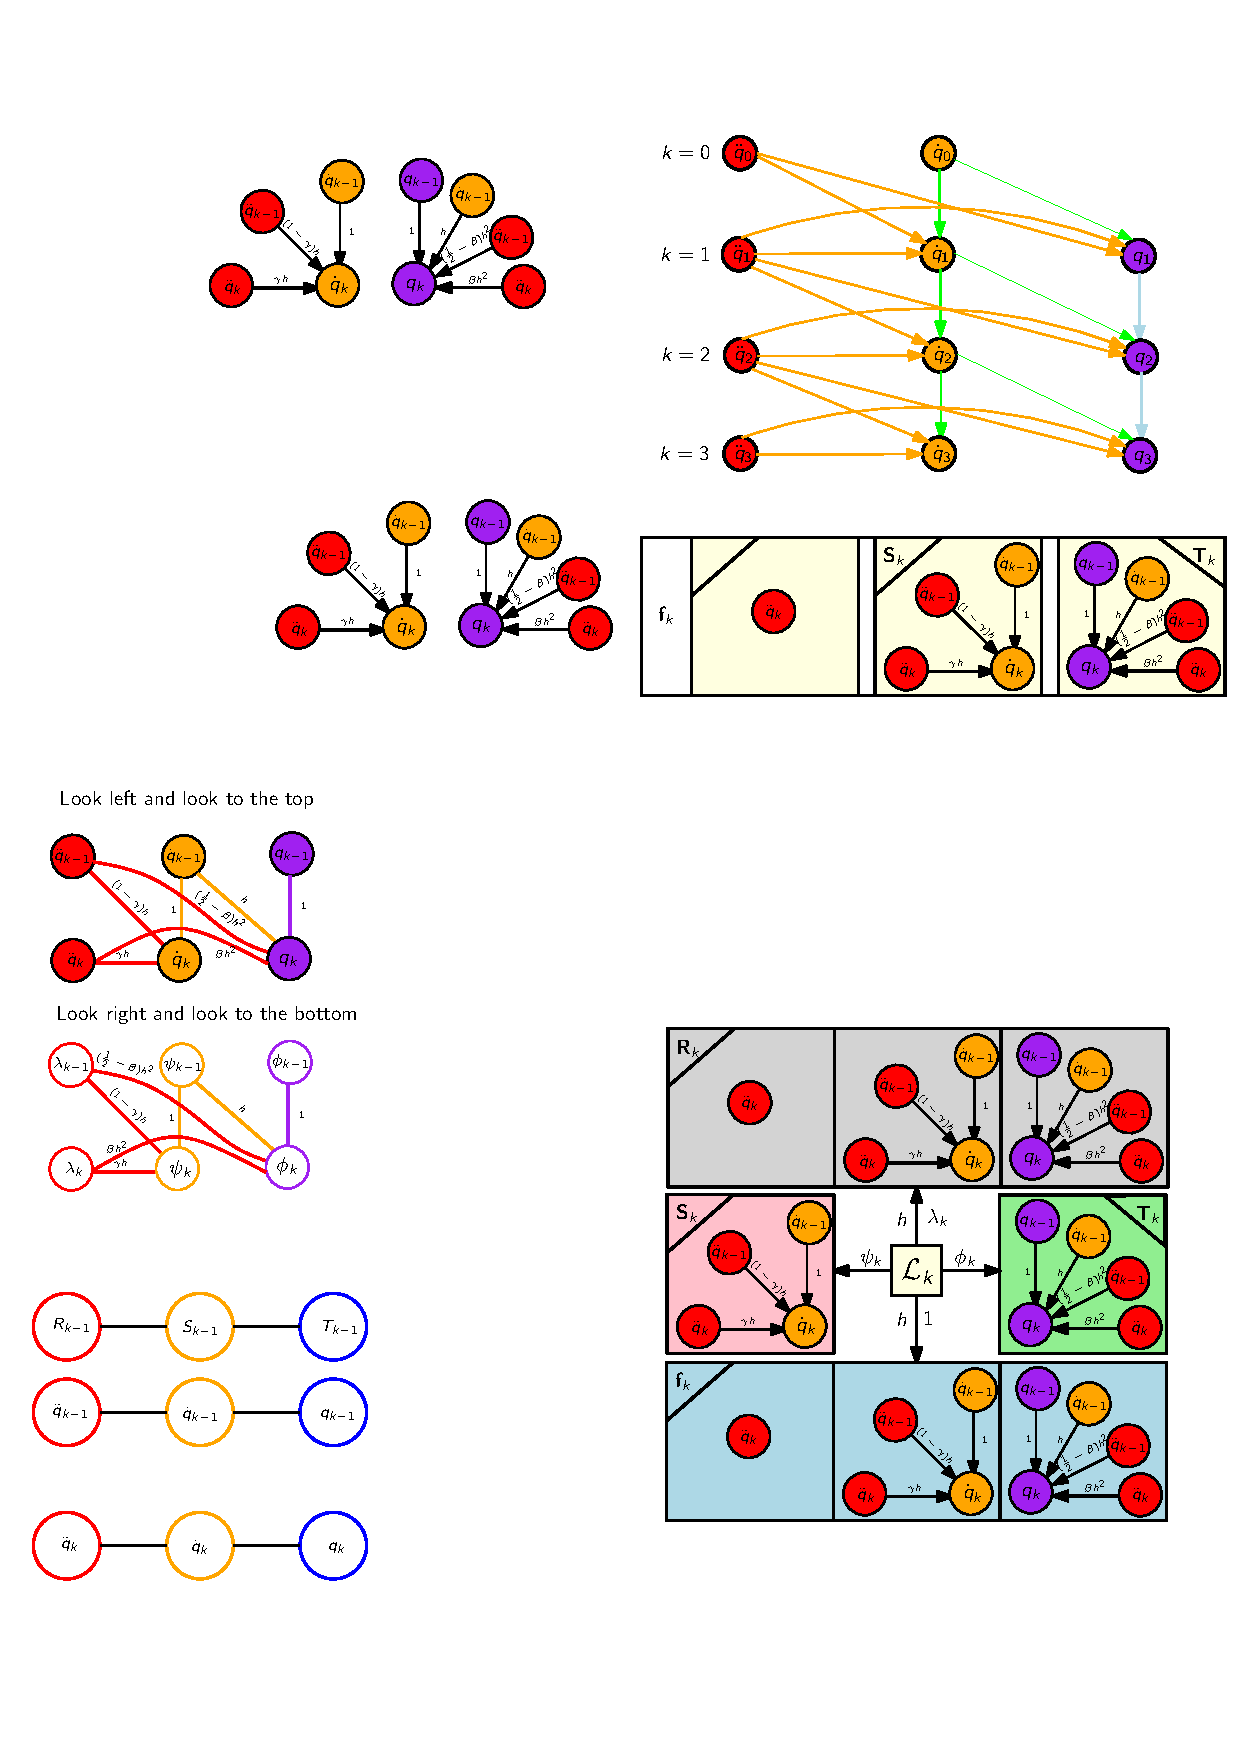
\includegraphics[width=\textwidth]{nbg-chart.pdf}
      %\caption{Illustrations showing the working of NBG method.}
      \label{fig:nbg-illustration}
    \end{figure}

    Setting $\pd{\cal{L}}{\ddot{q}_k} = 0$ yields:
    \begin{equation}
      \begin{split}
        \left[ \pd{R_k}{\ddot{q}_k} + \gamma h \pd{R_k}{\dot{q}_k} + \beta h^2 \pd{R_k}{{q}_k} \right]^T \rho_k = &- \left\{ \pd{f_k}{\ddot{q}_k} + \gamma h \pd{f_k}{\dot{q}_k} + \beta h^2 \pd{f_k}{{q}_k} \right\}^T \\
        & -  \frac{1}{h}\left\{  \gamma h  \sigma_k + \beta h^2   \tau_k \right\}^T\\
        & -  \left\{ (1-\gamma) h \pd{f_{k+1}}{\dot{q}_{k+1}} + \frac{1-2\beta}{2} h^2 \pd{f_{k+1}}{{q}_{k+1}} \right\}^T \\
        & -  \left[ (1-\gamma) h \pd{R_{k+1}}{\dot{q}_{k+1}} + \frac{1-2\beta}{2} h^2 \pd{R_{k+1}}{{q}_{k+1}} \right]^T\rho_{k+1} \\
        & -  \frac{1}{h} \left\{ (1-\gamma) h \sigma_{k+1} + \frac{1-2\beta}{2} h^2 \tau_{k+1} \right\}^T\\
      \end{split}
    \end{equation}
  }
\end{frame}
\end{noheadline}
\end{document}

%         We explore further simplifications by substituting equations.
%
%         \begin{equation}
%           \begin{split}
%             \left[ \frac{1}{h^2} \pd{R_k}{\ddot{q}_k} + \gamma \frac{1}{h} \pd{R_k}{\dot{q}_k} + \beta \pd{R_k}{{q}_k} \right]^T \rho_k = &- \left\{ \frac{1}{h^2}  \pd{f_k}{\ddot{q}_k} + \gamma \frac{1}{h} \pd{f_k}{\dot{q}_k} + \beta \pd{f_k}{{q}_k} \right\}^T \\
%             & -  \frac{1}{h}\left\{  \gamma \frac{1}{h}  \left( \sigma_{k+1} + h \tau_{k+1}  + \left\{ h \pd{f_{k+1}}{\dot{q}_{k+1}} +  h^2 \pd{f_{k+1}}{{q}_{k+1}} \right\}^T + \left[ h \pd{R_{k+1}}{\dot{q}_{k+1}} +  h^2 \pd{R_{k+1}}{{q}_{k+1}} \right]^T \rho_{k+1}  \right) \right\}^T \\
%             & -  \frac{1}{h}\left\{  \beta  \left( \tau_{k+1} + \left\{h \pd{f_{k+1}}{{q}_{k+1}} \right\}^T + \left[ h \pd{R_{k+1}}{{q}_{k+1}} \right]^T \rho_{k+1}  \right) \right\}^T\\
%             & -  \left\{ (1-\gamma) \frac{1}{h} \pd{f_{k+1}}{\dot{q}_{k+1}} + \frac{1-2\beta}{2} \pd{f_{k+1}}{{q}_{k+1}} \right\}^T \\
%             & -  \left[ (1-\gamma) \frac{1}{h} \pd{R_{k+1}}{\dot{q}_{k+1}} + \frac{1-2\beta}{2} \pd{R_{k+1}}{{q}_{k+1}} \right]^T\rho_{k+1} \\
%             & -  \frac{1}{h} \left\{ (1-\gamma) \frac{1}{h} \sigma_{k+1} + \frac{1-2\beta}{2} \tau_{k+1} \right\}^T\\
%           \end{split}
%         \end{equation}
%
%         \framebreak


         \framebreak
        
         Grouping the terms together we get:

         \begin{equation}
           \begin{split}
             \left[ \frac{1}{h^2} \pd{R_k}{\ddot{q}_k} + \gamma \frac{1}{h} \pd{R_k}{\dot{q}_k} + \beta \pd{R_k}{{q}_k} \right]^T \rho_k = &- \left\{ \frac{1}{h^2}  \pd{f_k}{\ddot{q}_k} + \gamma \frac{1}{h} \pd{f_k}{\dot{q}_k} + \beta \pd{f_k}{{q}_k} \right\}^T \\
             & -  \left\{  \gamma \frac{1}{h}  \pd{f_{k+1}}{\dot{q}_{k+1}} +  \gamma \pd{f_{k+1}}{{q}_{k+1}} \right\}^T \\ 
             & -  \left[  \gamma \frac{1}{h}  \pd{R_{k+1}}{\dot{q}_{k+1}} + \gamma \pd{R_{k+1}}{{q}_{k+1}} \right]^T \rho_{k+1}  \\
             & -  \left\{ \beta \pd{f_{k+1}}{{q}_{k+1}} \right\}^T \\ 
             & - \left[  \beta\pd{R_{k+1}}{{q}_{k+1}} \right]^T \rho_{k+1}  \\
             & -  \left\{ (1-\gamma) \frac{1}{h} \pd{f_{k+1}}{\dot{q}_{k+1}} + (\frac{1}{2}-\beta) \pd{f_{k+1}}{{q}_{k+1}} \right\}^T \\
             & -  \left[ (1-\gamma) \frac{1}{h} \pd{R_{k+1}}{\dot{q}_{k+1}} + (\frac{1}{2}-\beta) \pd{R_{k+1}}{{q}_{k+1}} \right]^T\rho_{k+1} \\
             & -  \frac{1}{h} \left\{ \frac{1}{h} \sigma_{k+1} + (\frac{1}{2} +\gamma) \tau_{k+1} \right\}^T\\
           \end{split}
         \end{equation}
        
         \begin{equation}
           \begin{split}
             \left[ \frac{1}{h^2} \pd{R_k}{\ddot{q}_k} + \gamma \frac{1}{h} \pd{R_k}{\dot{q}_k} + \beta \pd{R_k}{{q}_k} \right]^T \rho_k = &- \left\{ \frac{1}{h^2}  \pd{f_k}{\ddot{q}_k} + \gamma \frac{1}{h} \pd{f_k}{\dot{q}_k} + \beta \pd{f_k}{{q}_k} \right\}^T \\
             & -  \left\{  \frac{1}{h} \pd{f_{k+1}}{\dot{q}_{k+1}} +  (\frac{1}{2} +\gamma) \pd{f_{k+1}}{{q}_{k+1}} \right\}^T \\
             & -  \left[  \frac{1}{h} \pd{R_{k+1}}{\dot{q}_{k+1}} +  (\frac{1}{2} +\gamma)  \pd{R_{k+1}}{{q}_{k+1}} \right]^T\rho_{k+1} \\
             & -  \frac{1}{h} \left\{ \frac{1}{h} \sigma_{k+1} + (\frac{1}{2} +\gamma) \tau_{k+1} \right\}^T\\
           \end{split}
         \end{equation}

         Once the primary adjoint variables $\rho_k$ have been
         determined, the total derivative is readily obtained using
         Eq.\eqref{eqn:nbg-total-derivative}:
         $$\pd{\cal{L}}{x} = \pd{F}{x} = \sum_{k=0}^N h \pd{f_k}{x}^T
         + \sum_{k=0}^N h \pd{R_k}{x}^T \rho_k.$$ Notice that
         $\pd{S_k}{x} = \pd{T_k}{x} = 0$.  
  


         We can equivalently scale the equation with $1/h^2$ and represent as follows:
         
         \begin{equation}
           \begin{split}
             \left[ \frac{1}{h^2} \pd{R_k}{\ddot{q}_k} + \gamma \frac{1}{h} \pd{R_k}{\dot{q}_k} + \beta \pd{R_k}{{q}_k} \right]^T \rho_k = &- \left\{ \frac{1}{h^2}  \pd{f_k}{\ddot{q}_k} + \gamma \frac{1}{h} \pd{f_k}{\dot{q}_k} + \beta \pd{f_k}{{q}_k} \right\}^T \\
             & -  \frac{1}{h}\left\{  \gamma \frac{1}{h}  \sigma_k + \beta   \tau_k \right\}^T\\
             & -  \left\{ (1-\gamma) \frac{1}{h} \pd{f_{k+1}}{\dot{q}_{k+1}} + \frac{1-2\beta}{2} \pd{f_{k+1}}{{q}_{k+1}} \right\}^T \\
                          & -  \left[ (1-\gamma) \frac{1}{h} \pd{R_{k+1}}{\dot{q}_{k+1}} + \frac{1-2\beta}{2} \pd{R_{k+1}}{{q}_{k+1}} \right]^T\rho_{k+1} \\
             & -  \frac{1}{h} \left\{ (1-\gamma) \frac{1}{h} \sigma_{k+1} + \frac{1-2\beta}{2} \tau_{k+1} \right\}^T\\
           \end{split}
         \end{equation}
